\begin{tcolorbox}[colback=violet!5!white,colframe=violet!75!black,title=\textbf{Direct
    Approach}]
\textbf{Direct single shooting:} corresponds to sequential approach\\
\begin{center}
  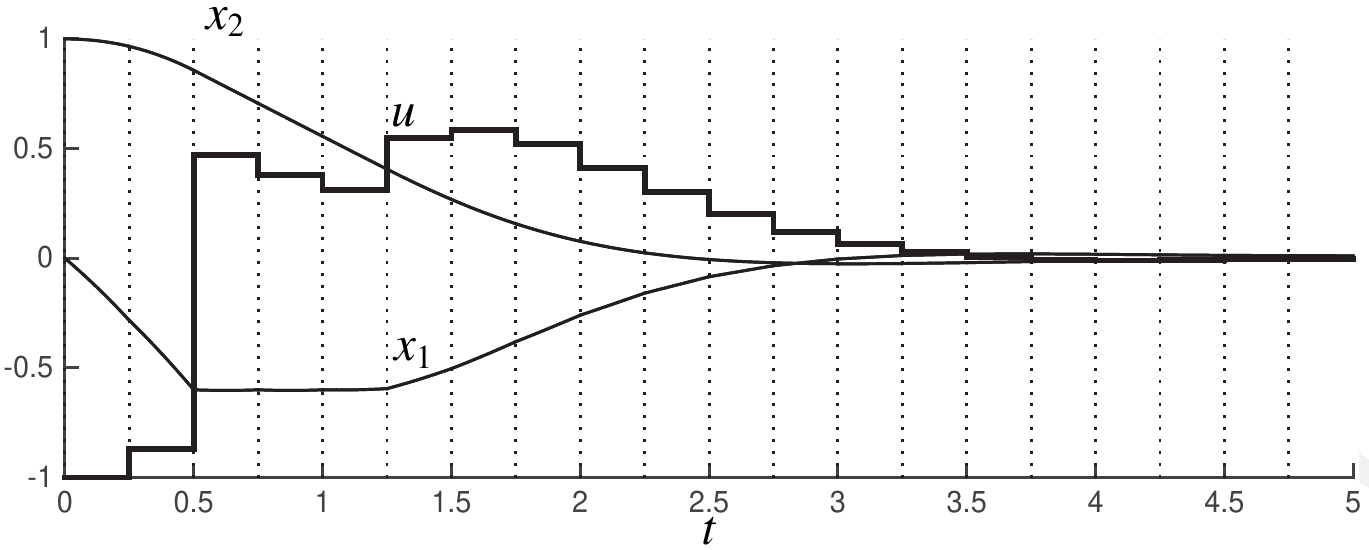
\includegraphics[width=0.8\textwidth]{direct_single_shooting}
\end{center}

  \begin{itemize}
  \item parametrize control function $u(t)$ into $N$ timesteps (polynomial of
    $n$-th grade, mostly $n=0$):
    \[u(t,q)=q_k,\quad t=[t_k,t_{k+1}],\quad q\in \mathbb{R}^N\]
  \item Forward simulate system dynamics
  \item Lower triangular jacobian of inequ. constraints
  \item Dense Hessian of Lagrange function
  \item Very good initial guess for $q$ required (difficult)\\
  \end{itemize}
  
\textbf{Direct multiple shooting:} corresponds to simultaneous approach\\
\begin{center}
  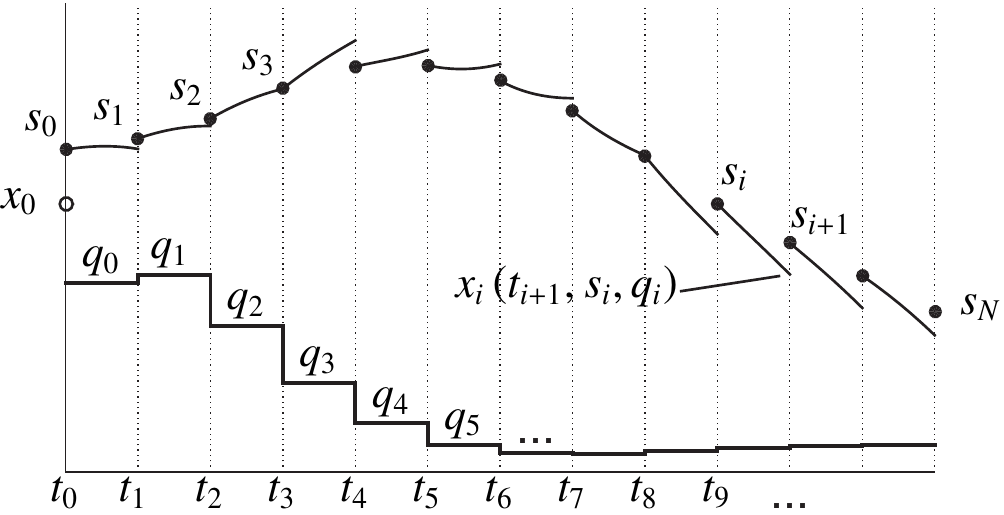
\includegraphics[width=0.8\textwidth,height=25mm]{direct_multiple_shooting}
\end{center}

  \begin{itemize}
  \item Same parametrisation as in single shooting
  \item Solve the ODE separately on each interval $[t_i,t_{i+1}]$:
    \begin{align*}
      \dot{x}_i(t, s_i, u_i) &= f(x_i(t,s_i,q_i),q_i) \\
      x_i(t_i,s_i,u_i) &= s_i
    \end{align*}
  \item Numerically integrate the cost over all intervals
  \item Additional continuity condition (piecing results together --- entails
    the system dynamics $f(x(t),u(t))$):
    \[s_{i+1}=x_i(t_{i+1},s_i,u_i)\]
  \item Eq. constraint ordering important (init. val.,
    continuity, path constr.) for sparsity structure
  \end{itemize}
  \textbf{Direct collocation:} Approximate states with polynomials\\
  \begin{itemize}
  \item Parametrize $u(t)$ again (here: constant, i.e. $u(t)=q_k, t\in [t_k,t_{k+1}]$)
  \item Create polynomial fits $p_k(t, v_k)\in \mathbb{R}$ for each timestep $t_k$.
  \item Collocation equation (fitting system dynamics):
    \[c_k(v_k,s_k,q_k)=
      \left[
        \begin{array}{c}
          v_{k,0}-s_k \\
          \dot{p_k}(t_{k,1},v_k) - f(v_{k,1}, q_k) \\
          \vdots \\
          \dot{p_k}(t_{k,d},v_k) - f(v_{k,d}, q_k) \\
        \end{array}
      \right]=0,
      \quad
      \begin{array}{c}
        v_{k,i}\in \mathbb{R}^{n_x}\\
        i=0, \dots, d
      \end{array}
    \]
  \item Integrate $L$: $l_k(v_k,s_k,q_k) := \int^{t_{k+1}}_{t_k} L(x,u)\mathrm{d}t$
\item Collocation NLP:
\[
  \begin{array}{rrl}
    \min_{v,s,q}&\quad  E(s_N) + &\sum^{N-1}_{k=0} l_k(v_k,s_k,q_k) \\
    \mathrm{s.t.}&\quad s_0 - x_0 &= 0\quad \mathrm{(initial\ state)} \\
    &c_k(v_k,s_k,q_k) &= 0 \quad \mathrm{(collocation\ conditions)} \\ 
    &p_k(t_{k+1},v_k) - s_{k+1} &= 0\quad \mathrm{(continuity\ conditions)} \\
    &h(s_k,q_k)&\le 0\quad \mathrm{(path\ constraints)} \\
    & r(s_N) &\le 0\quad \mathrm{(terminal\ state)}
  \end{array}
\]
  \end{itemize}
\end{tcolorbox}
%%% Local Variables:
%%% mode: latex
%%% TeX-master: "../HelpSheet"
%%% TeX-engine: xetex
%%% End:
